%%%%%%%%%%%%%%%%%%%%%%%%%%%%%%%%%%%%%%%%%
% Journal Article
% LaTeX Template
% Version 1.4 (15/5/16)
%
% This template has been downloaded from:
% http://www.LaTeXTemplates.com
%
% Original author:
% Frits Wenneker (http://www.howtotex.com) with extensive modifications by
% Vel (vel@LaTeXTemplates.com)
%
% License:
% CC BY-NC-SA 3.0 (http://creativecommons.org/licenses/by-nc-sa/3.0/)
%
%%%%%%%%%%%%%%%%%%%%%%%%%%%%%%%%%%%%%%%%%

%----------------------------------------------------------------------------------------
%	PACKAGES AND OTHER DOCUMENT CONFIGURATIONS
%----------------------------------------------------------------------------------------

\documentclass[twoside,twocolumn]{article}

\usepackage{blindtext} % Package to generate dummy text throughout this template 

\usepackage[sc]{mathpazo} % Use the Palatino font
\usepackage[T1]{fontenc} % Use 8-bit encoding that has 256 glyphs
\linespread{1.05} % Line spacing - Palatino needs more space between lines
\usepackage{microtype} % Slightly tweak font spacing for aesthetics

\usepackage[english]{babel} % Language hyphenation and typographical rules

\usepackage[hmarginratio=1:1,top=32mm,columnsep=20pt]{geometry} % Document margins
\usepackage[hang, small,labelfont=bf,up,textfont=it,up]{caption} % Custom captions under/above floats in tables or figures
\usepackage{booktabs} % Horizontal rules in tables

\usepackage{lettrine} % The lettrine is the first enlarged letter at the beginning of the text

\usepackage{enumitem} % Customized lists
\setlist[itemize]{noitemsep} % Make itemize lists more compact

\usepackage{abstract} % Allows abstract customization
\renewcommand{\abstractnamefont}{\normalfont\bfseries} % Set the "Abstract" text to bold
\renewcommand{\abstracttextfont}{\normalfont\small\itshape} % Set the abstract itself to small italic text

\usepackage{titlesec} % Allows customization of titles
\renewcommand\thesection{\Roman{section}} % Roman numerals for the sections
\renewcommand\thesubsection{\roman{subsection}} % roman numerals for subsections
\titleformat{\section}[block]{\large\scshape\centering}{\thesection.}{1em}{} % Change the look of the section titles
\titleformat{\subsection}[block]{\large}{\thesubsection.}{1em}{} % Change the look of the section titles

\usepackage{fancyhdr} % Headers and footers
\pagestyle{fancy} % All pages have headers and footers
\fancyhead{} % Blank out the default header
\fancyfoot{} % Blank out the default footer
\fancyhead[C]{5584F $\bullet$ December 2019 $\bullet$ 4M20} % Custom header text
\fancyfoot[RO,LE]{\thepage} % Custom footer text

\usepackage{titling} % Customizing the title section

\usepackage{hyperref} % For hyperlinks in the PDF

\usepackage{graphicx}
\graphicspath{ {images/} }

\newenvironment{reusefigure}[2][htbp]
  {\addtocounter{figure}{-1}%
   \renewcommand{\theHfigure}{dupe-fig}% If you're using hyperref
   \renewcommand{\thefigure}{\ref{#2}}% Figure counter is \ref
   \renewcommand{\addcontentsline}[3]{}% Avoid placing figure in LoF
   \begin{figure}[#1]}
  {\end{figure}}
\usepackage{wrapfig}
\usepackage{amsmath}
\usepackage{xcolor}
\usepackage{listings}
\usepackage{subcaption}
\usepackage{pdfpages}
\usepackage{array,multirow,graphicx}
\lstset{
  basicstyle=\ttfamily,
  columns=fullflexible,
  frame=single,
  breaklines=true,
  postbreak=\mbox{\textcolor{red}{$\hookrightarrow$}\space},
}

\newcommand{\threepartdef}[6]
{
	\left\{
		\begin{array}{lll}
			#1 & \mbox{: } #2 \\
			#3 & \mbox{: } #4 \\
			#5 & \mbox{: } #6 \\
			0 & \mbox{: } otherwise
		\end{array}
	\right.
}
%----------------------------------------------------------------------------------------
%	TITLE SECTION
%----------------------------------------------------------------------------------------

\setlength{\droptitle}{-4\baselineskip} % Move the title up

\pretitle{\begin{center}\Huge\bfseries} % Article title formatting
\posttitle{\end{center}} % Article title closing formatting
\title{4M20 - Coursework Two} % Article title
\author{%
\\
\textsc{Candidate Number: 5584F}% Your email address
}
\date{\today} % Leave empty to omit a date
\renewcommand{\maketitlehookd}{%
\begin{abstract}
\noindent
Three link robots are extremely versatile and can be used in applications ranging from robotic arms to moving robots. Throughout this investigation a three link walker robot was tasked with traversing a pre-determined terrain involving stairs. Kinematic control was considered for the majority of tasks due to the decreased complexity in computation compared to a dynamic model. The robot consists of three joints that move around 2D space, this creates lots of options for path trajectory which can be optimised to suit different conditions and constraints. Changes were required to make the robot suitable for the task. The robot was ultimately unable to fully complete the task, so various additional were considered to complete it.
\end{abstract}
}
%----------------------------------------------------------------------------------------

\begin{document}
\onecolumn
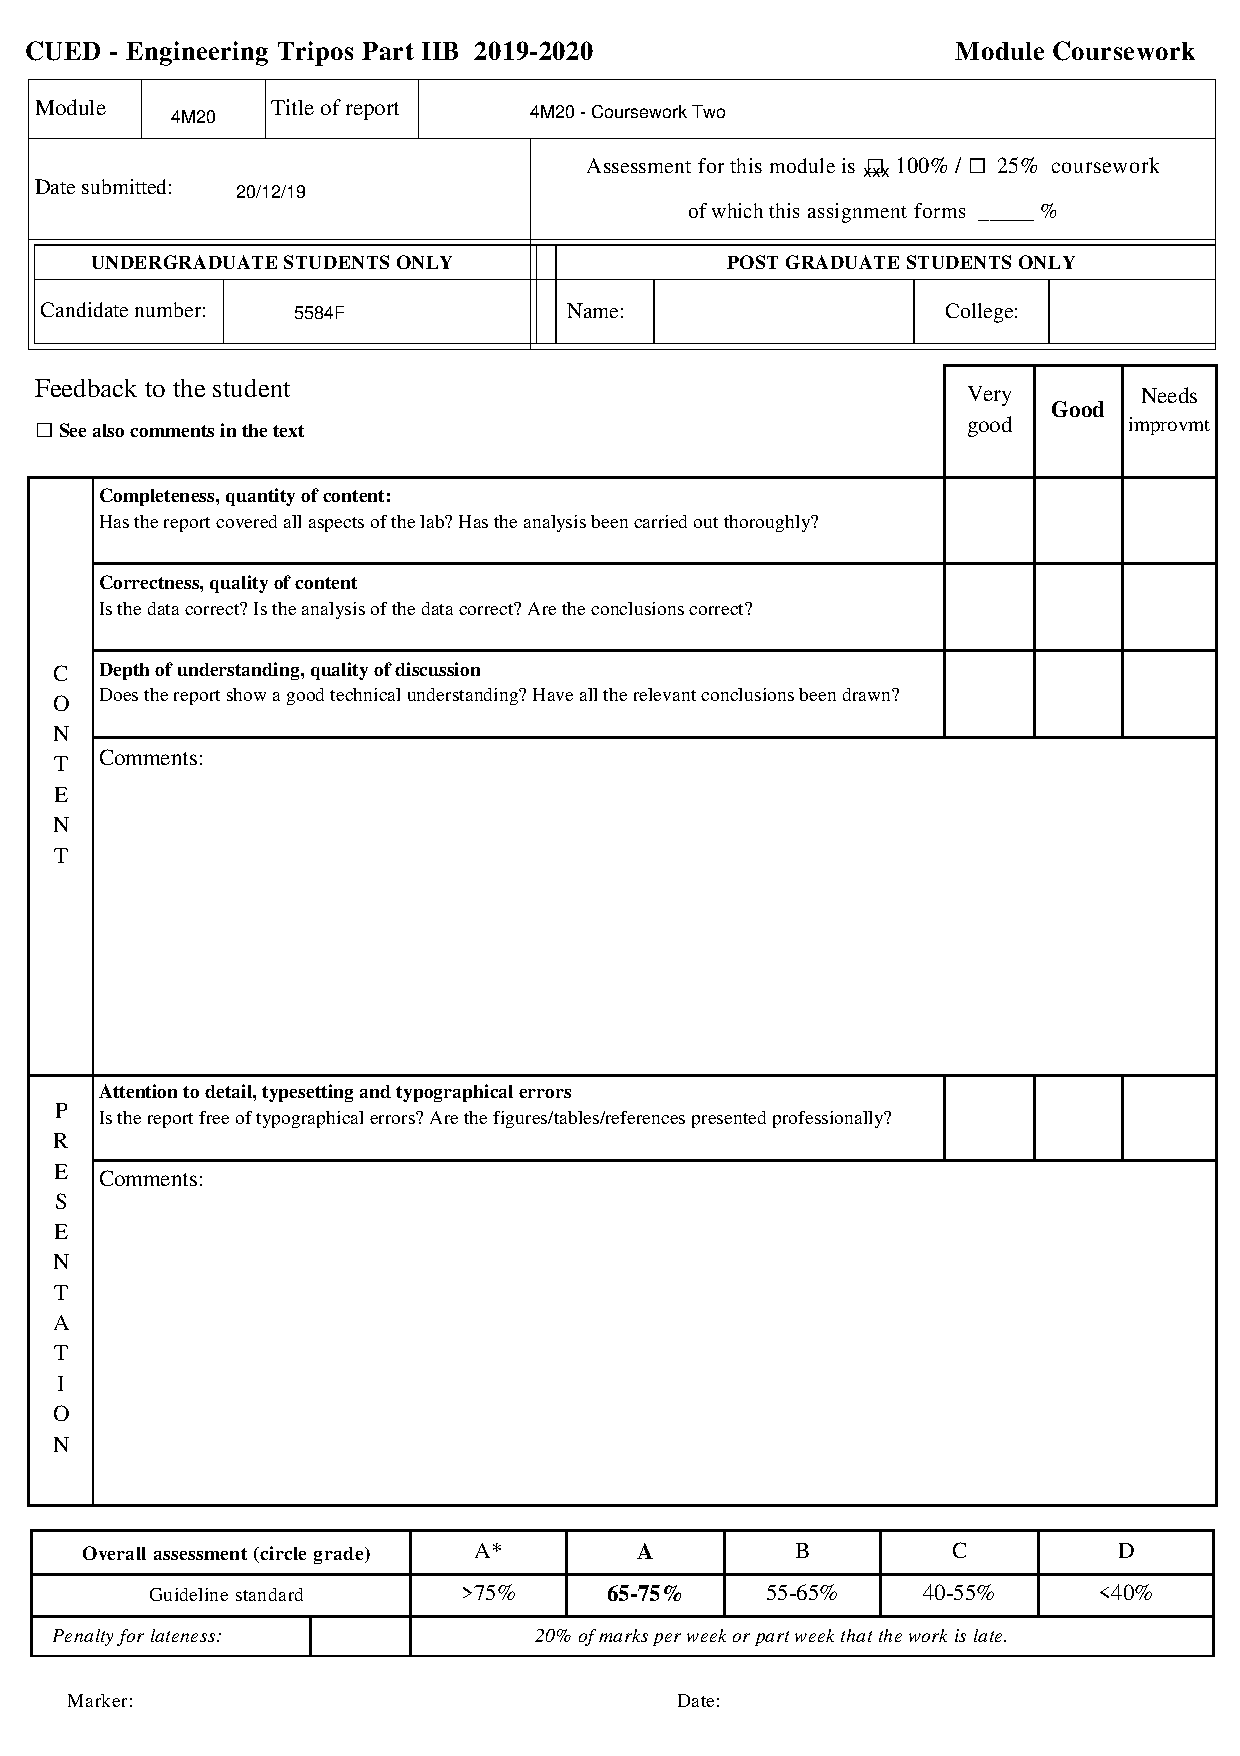
\includepdf[pages={1}]{Coversheet.pdf}
\twocolumn
\pagenumbering{arabic}
% Print the title
\maketitle

%----------------------------------------------------------------------------------------
%	ARTICLE CONTENTS
%----------------------------------------------------------------------------------------

\section{Introduction}

\lettrine[nindent=0em,lines=3]{T}heoretical and numeric investigations of a 3 link walking robot are described in this report. The robot analysed is shown in figure \ref{fig:diagram} and is designed to traverse the terrain shown in figure \ref{fig:ter}.	

\begin{figure}[h]
  \centering
    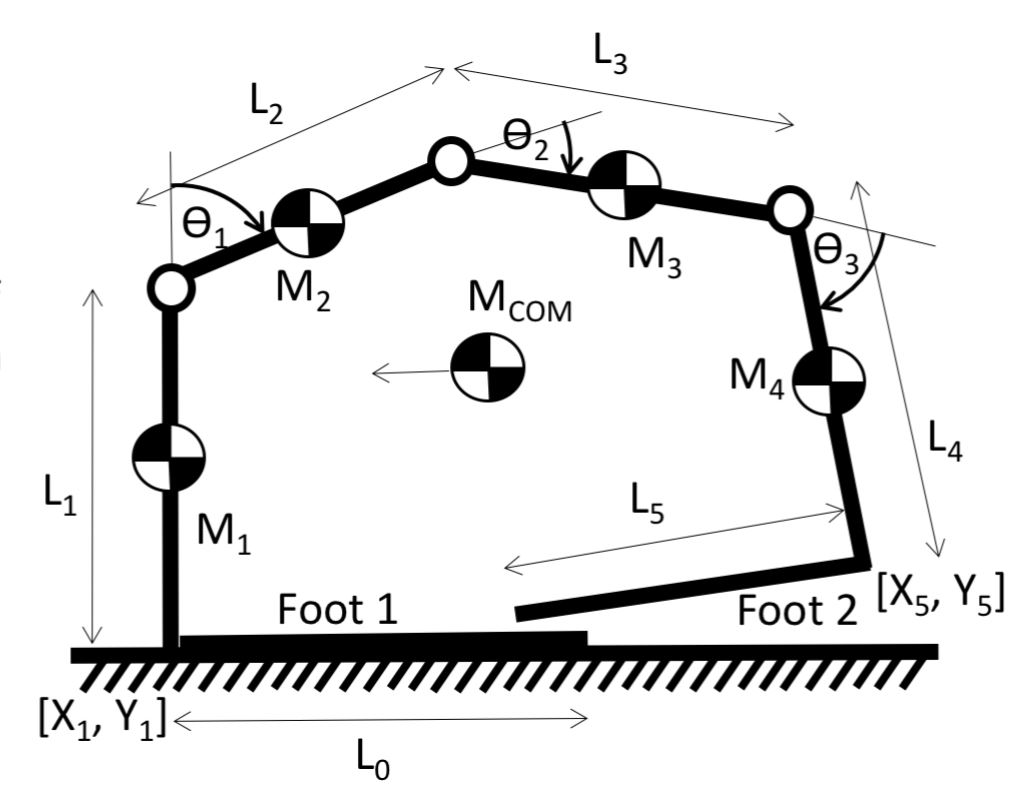
\includegraphics[width=\linewidth]{diagram}
  \caption{Diagram of robotic walker}
  \label{fig:diagram}
\end{figure}

\begin{figure}[h]
  \centering
    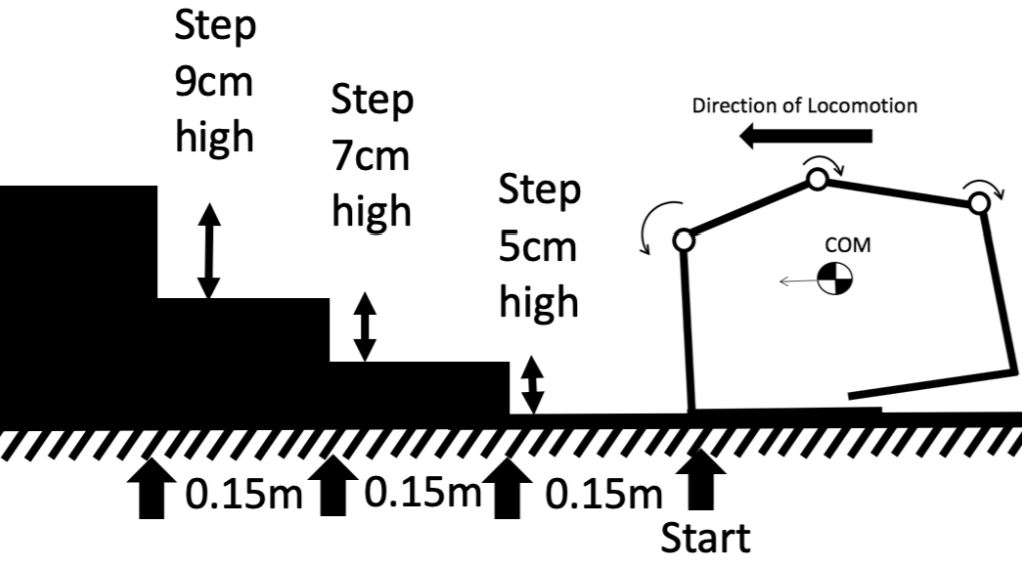
\includegraphics[width=\linewidth]{terrain}
  \caption{Terrain to be traversed by the robot}
  \label{fig:ter}
\end{figure}
%------------------------------------------------

\section{Question 1}
\subsection{Kinematics}
When one foot of the robot is fixed, the robot becomes a three degree of freedom system with variables: $\boldsymbol{\theta}=[\theta_1,\theta_2, \theta_3]^T$. However, the output is only of degree two: \textbf{X}=$[X_5,Y_5]^T$, which leads to a variety of kinematic solutions. When the orientation of link 4 is considered it becomes a 3 DoF output. Forward kinematics can be used to convert the joint position $\boldsymbol{\theta}$ into moving foot position \textbf{X}, with inverse kinematics doing the reverse. Using the angles and lengths defined in figure \ref{fig:diagram} the forward kinematics in equation \ref{eq:fk} is calculated, or as in equation \ref{eq:fk2} when foot 1 is being lifted. The forward kinematic equations can then be used to find solutions of $\boldsymbol{\theta}$ that give a desired foot position.
\newline
To achieve a foot 2 position of [0.15m,0.15m] when all lengths = 0.1m results in lots of viable joint angles as shown in figures \ref{fig:angles} and \ref{fig:pos1} and table \ref{table:ang}. Multiple solutions exist because the orientation of $L_4$ is undefined in this problem. If we choose to define this orientation we can obtain a simple result. To get a foot 2 position of [0.12m,0m] with link 4 vertical the joint angles $\boldsymbol{\theta} = [36.87,106.3,36.87]$ are required as shown in figure \ref{fig:pos2}.

\begin{figure}[h]
  \centering
    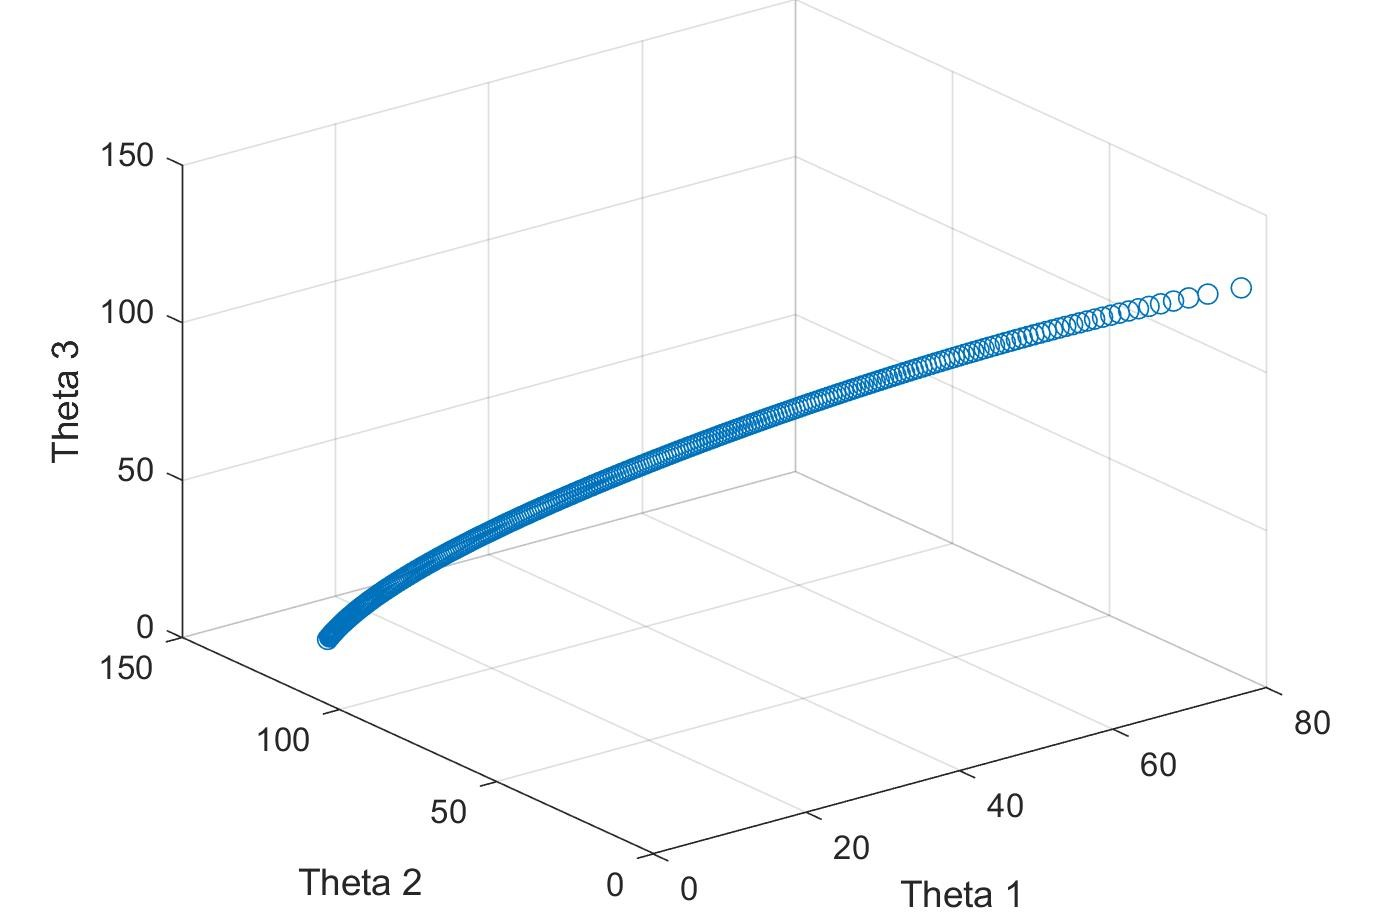
\includegraphics[width=\linewidth]{1_1}
  \caption{Some possible joint angles to achieve $[x_5,y_5]=[0.15,0.15]$}
  \label{fig:angles}
\end{figure}


\begin{figure}[h]
  \centering
    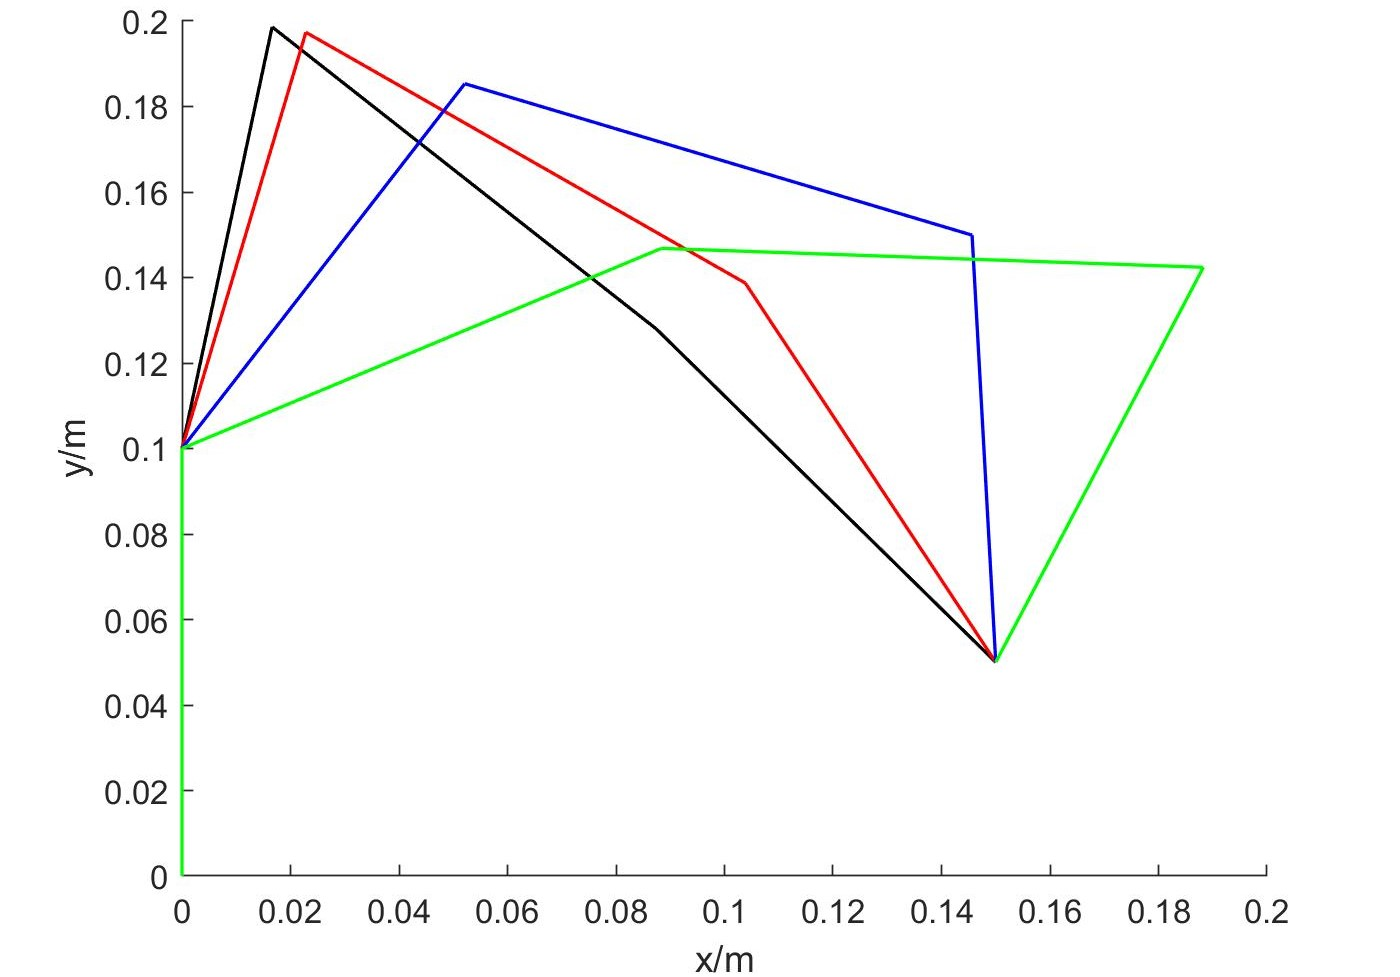
\includegraphics[width=\linewidth]{pos1}
  \caption{Drawing of joint angles for $[x_5,y_5]=[0.15,0.15]$}
  \label{fig:pos1}
\end{figure}

\begin{table}[h]
\centering 
\begin{tabular}{ c | c | c }
$\theta_1$&$\theta_2$&$\theta_3$\\ 

\midrule
10.69&119.9&15.62\\
24.84&90.16&55\\
42.44&61.94&83.87\\
59.87&34.14&107.2\\
\end{tabular}
\caption{Example angles for $[x_5,y_5]=[0.15,0.15]$}
\label{table:ang}
\end{table}

\begin{figure}[h]
  \centering
    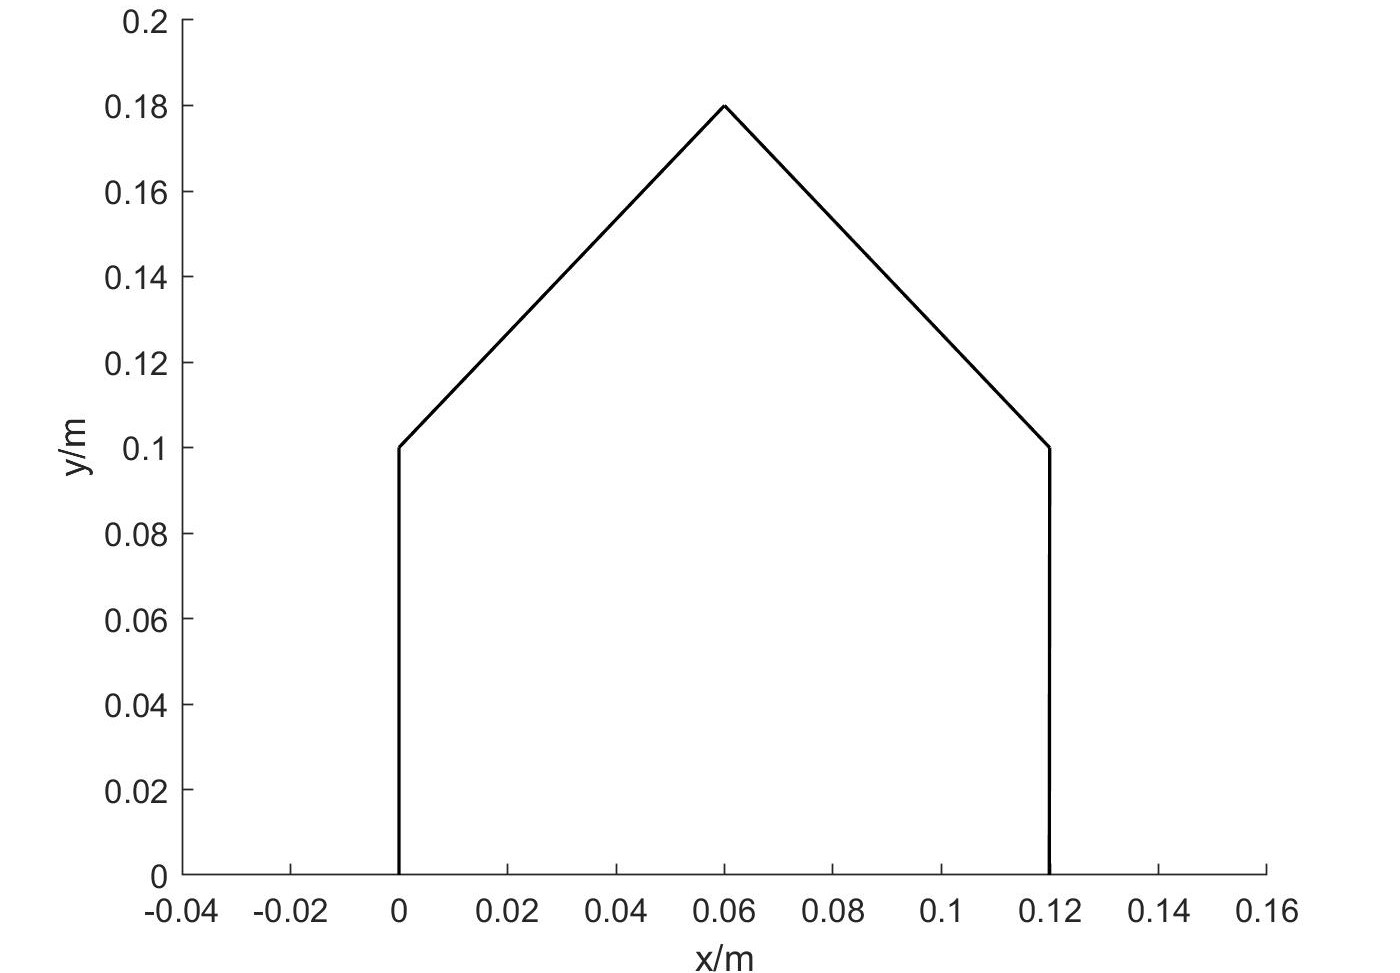
\includegraphics[width=\linewidth]{pos2}
  \caption{Joint angles required for foot position [0.12m,0m]}
  \label{fig:pos2}
\end{figure}
\subsection{Centre of Mass}
The centre of mass of the robot is very important as this must reside above the stationary foots base in order for the robot to not topple. The centre of mass can be calculated using equation \ref{eq:com} and approximating the robots components as point masses, only $x_{com}$ is required to check stability. Ensuring the robot doesn't topple is essential as it means the problem can be solved using just kinematics. Without toppling the ground foot can be assumed to be fixed meaning all positions are defined from the kinematic equations \ref{eq:fk} or \ref{eq:fk2}. When solving a kinematic equation the forces and accelerations aren't considered. This vastly simplifies the problem compared to dynamic methods. 
\begin{equation}
\begin{split}
x_{com} = \frac{\sum_i m_i x_i}{\sum_i m_i}\\
y_{com} = \frac{\sum_i m_i y_i}{\sum_i m_i}\\
\end{split}
\label{eq:com}
\end{equation} 




%------------------------------------------------
\section{Question 2}
\subsection{Joint Planning Algorithm}
To develop a walking robot the joint trajectories throughout motion are required. These joint trajectories are calculated in real time for a given stride length and robot geometry. The walking was made of five intermediate stages as shown in figure \ref{fig:steps}, these are asymmetric to improve stability. The stage positions are determined by calculating each foot position in the stages based off the required stride length. Inverse kinematics was then used to determine the joint angles at these positions. Third order polynomial fitting is then used to interpolate between stages smoothly. Each stage could take a variable amount of time to further allow optimisation.
\newline
Computational speed was essential for solving inverse kinematics equations in real time. For this we used fsolve in MatLab, with link one and four kept vertical. Fsolve returns the nearest single solution to an initial guess, which was the last stage position. This ensured that the total joint movement between stages was minimised and therefore reducing energy use. Fsolve also allowed unreachable stride lengths to not cause errors.

\begin{figure}[h]
  \centering
  \begin{subfigure}[t]{0.5\textwidth}
    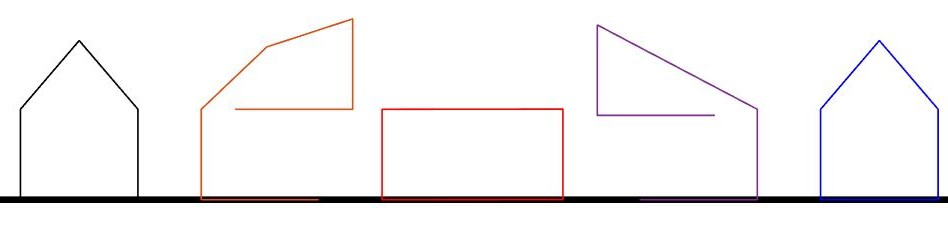
\includegraphics[width=\linewidth]{15cm}
  \caption{15cm}
  \label{fig:steps}
  \end{subfigure}
  \begin{subfigure}[t]{0.5\textwidth}
    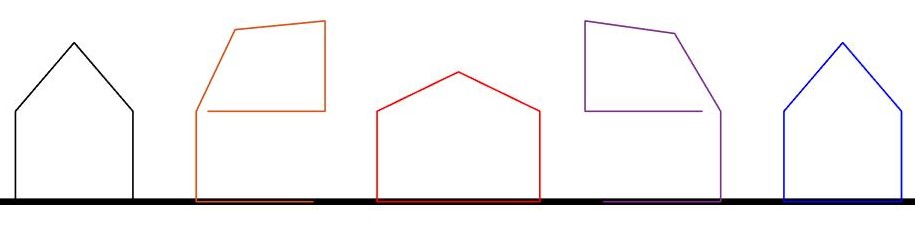
\includegraphics[width=\linewidth]{5cm}
  \caption{5cm}
  \label{fig:stages2}
  \end{subfigure}
  \caption{Intermediate stages for a given stride length}
  \label{fig:st}
\end{figure}

A 15cm Stride is not possible with the link lengths given in the brief. In figure \ref{fig:steps} this is shown by the step stages requiring fully extended top links. Reducing the stride length to 5cm changes the positions to figure \ref{fig:stages2}. This change improves the stability of the robot.
\newline
In order to reduce forces exerted on the robot by smoothing joint accelerations and velocities third order polynomial interpolation is used between stages. Figure \ref{fig:jt} shows the joint trajectories for one 5cm step. The plots show a smooth curve with small plateau at the location of each defined stage from figure \ref{fig:stages2}. The maximum $\boldsymbol{\dot{\theta}}$ and $\boldsymbol{\ddot{\theta}}$ are shown in table \ref{table:max}.

\begin{figure}[h]
  \centering
    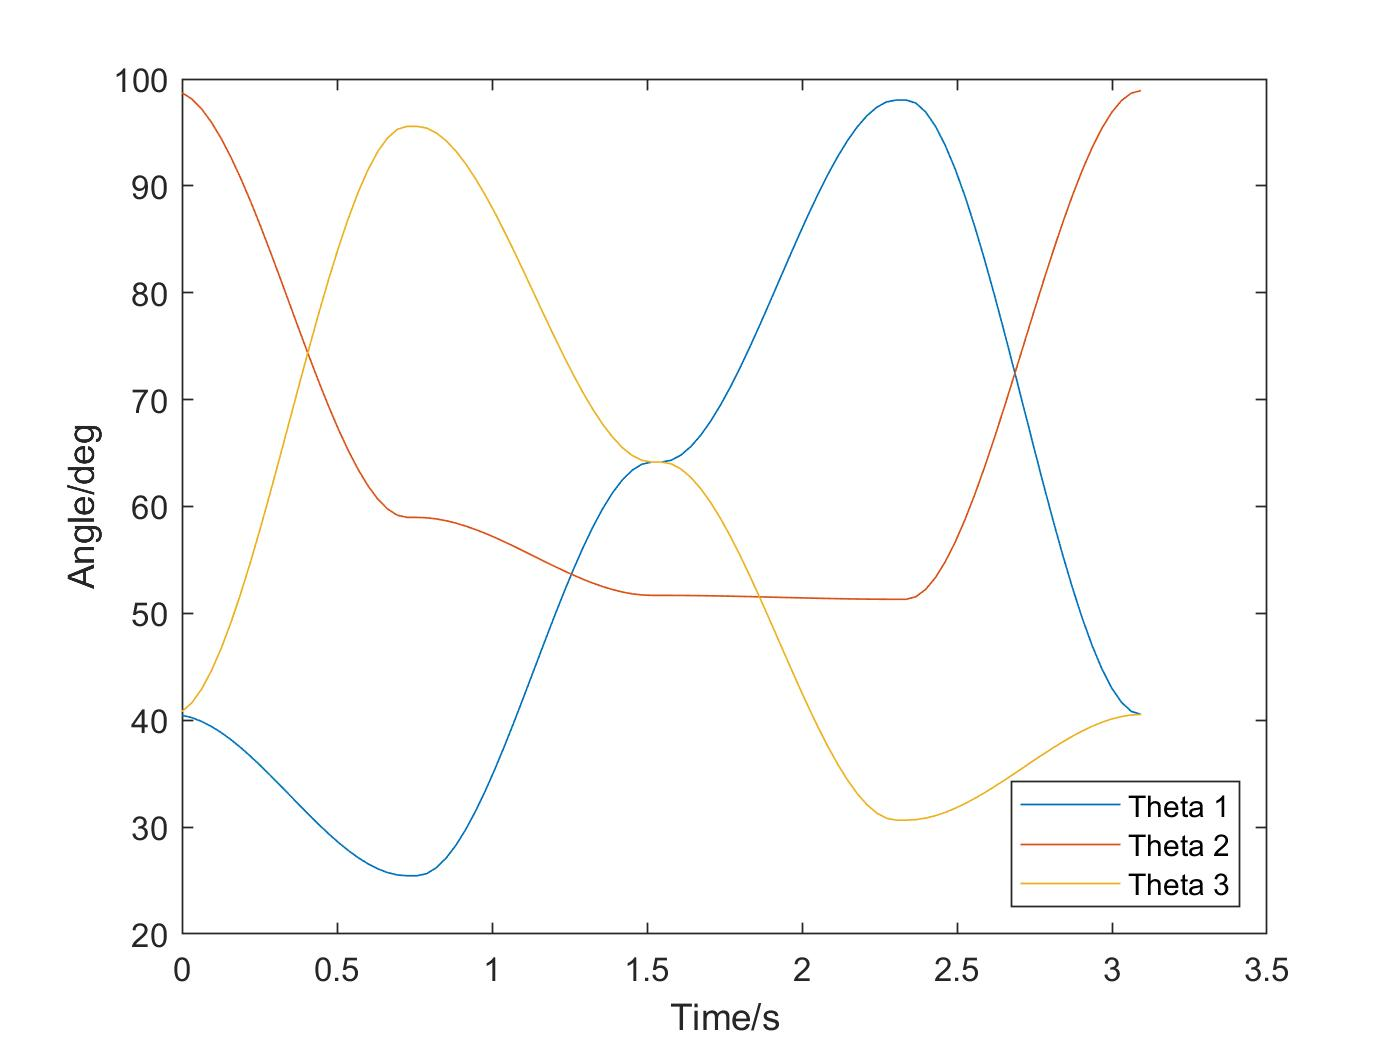
\includegraphics[width=\linewidth]{5cmtraj}
  \caption{Joint angle trajectories for a 5cm stride}
  \label{fig:jt}
\end{figure}


\begin{table}[h]
\centering 
\begin{tabular}{ c | c | c }
Joint&|$\dot{\theta}_{max}$|&|$\ddot{\theta}_{max}$|\\ 

\midrule
1&114.7&562.1\\
2&95.0&465.4\\
3&109.8&538.0\\
\end{tabular}
\caption{Maximum $\boldsymbol{\dot{\theta}}$ and $\boldsymbol{\ddot{\theta}}$ for a 5cm step}
\label{table:max}
\end{table}

At each position throughout the motion the centre of mass can be calculated to check the robot will remain stable. If it's not stable through the whole motion tweaks to the position can be easily made. 


%------------------------------------------------
\section{Question 3}
\subsection{Changes required} 
When implementing the joint trajectories for stepping onto the real robot several changes were required to increase the reliability of the robot. These changes were as follows:
\begin{itemize}
\item Convert angles to work with the hardware using equation \ref{eq:con} 

\item Increase the friction of the feet using blue tac and rubber bands
\item Increase foot stiffness to reduce bending
\item Change the desired orientation of the leading foot to not be vertical, to account for the bending of the robot
\item  Asymmetric step stages to increase stability, due to COM calculations not being accurate enough on the real robot
\end{itemize}
Lots of these changes were to make real life more similar to the idealised simulation.

\begin{equation}
\begin{bmatrix}
p_1 \\
p_2 \\
p_3
\end{bmatrix}
=
\begin{bmatrix}
\theta_1 + 7 \\
\theta_2 + 7 \\
140-\theta_3
\end{bmatrix}/160
\label{eq:con}
\end{equation}

\subsection{Performance}
Implementing a 15cm step was now theoretically possible with the robot due the length changes. However due to bending, slip and slight wobble present in the robot a 15cm step wasn't achieved in practice. Across 10 steps our robot moved an average of 87.6mm with standard deviation 1.84mm. While this wasn't the stride length required it was repeatable. This repeatability ensured that we were able to take consistent steps and account for the under step.
\subsection{Dynamics model}
A dynamics model can be formed as in equations \ref{eq:dyn}. The dynamics model takes the current robot state $\boldsymbol{X_{k}} = [X_k, dX_k]^T$ after k steps and calculates the state an additional step for a given input $\boldsymbol{u_k}$. The state is comprised of $X_k$ which is the x-coordinate of the back foot, and $dX_k$ which is the distance between front and back leg at the stationary stance. The inputs are $\boldsymbol{u_k} = [Stride \: length, Next \: stance]^T$ and determine how large the next step will be and what position the robot should end up in. In the model there is a process noise term with mean $\boldsymbol{\mu}$ and standard deviation $\boldsymbol{\sigma}$, this is to account for uncertainty in movements and drift observed in real life due to factors such as bending.

\begin{equation}
\begin{split}
\boldsymbol{X_{k+1}} = \boldsymbol{AX_k}+\boldsymbol{Bu_k} + \boldsymbol{n_k}\\
\boldsymbol{A} =
\begin{bmatrix}
1  0 \\
0  0 \\
\end{bmatrix}, \: \boldsymbol{B}=
\begin{bmatrix}
1  0 \\
0  1 \\
\end{bmatrix}\\
\boldsymbol{n_k} \sim \mathcal{N}(\boldsymbol{\mu},\boldsymbol{\sigma}) \\
\end{split}
\label{eq:dyn}
\end{equation}

\subsection{Kalman-filter}
The uncertainty in stepping builds up as time advances. This increases the chance that the robot will not be successful at the task. The robot loses the ability to reliably move a given distance, or balance on a step when this uncertainty in position is present. To solve this problem a feedback system using sensors and state estimation can be implemented.
\newline
To better estimate the true position and avoid errors building up sensors are required. These are to measure the distance to the next step and distance between both legs. These two variables make up the state vector $\boldsymbol{X_k}$. State measurement has uncertainty associated with it, for this reason measuring the state gives an estimated position with a certain covariance.
\newline
By Implementing a Kalman filter algorithm the state distribution given by the dynamics model in equation \ref{eq:dyn} can be updated to form a posterior estimate containing the new information from state observation as in figure \ref{fig:kal}. These updates occur after each step the robot takes, and help to build a more accurate dynamic model.

\begin{figure}[h]
  \centering
    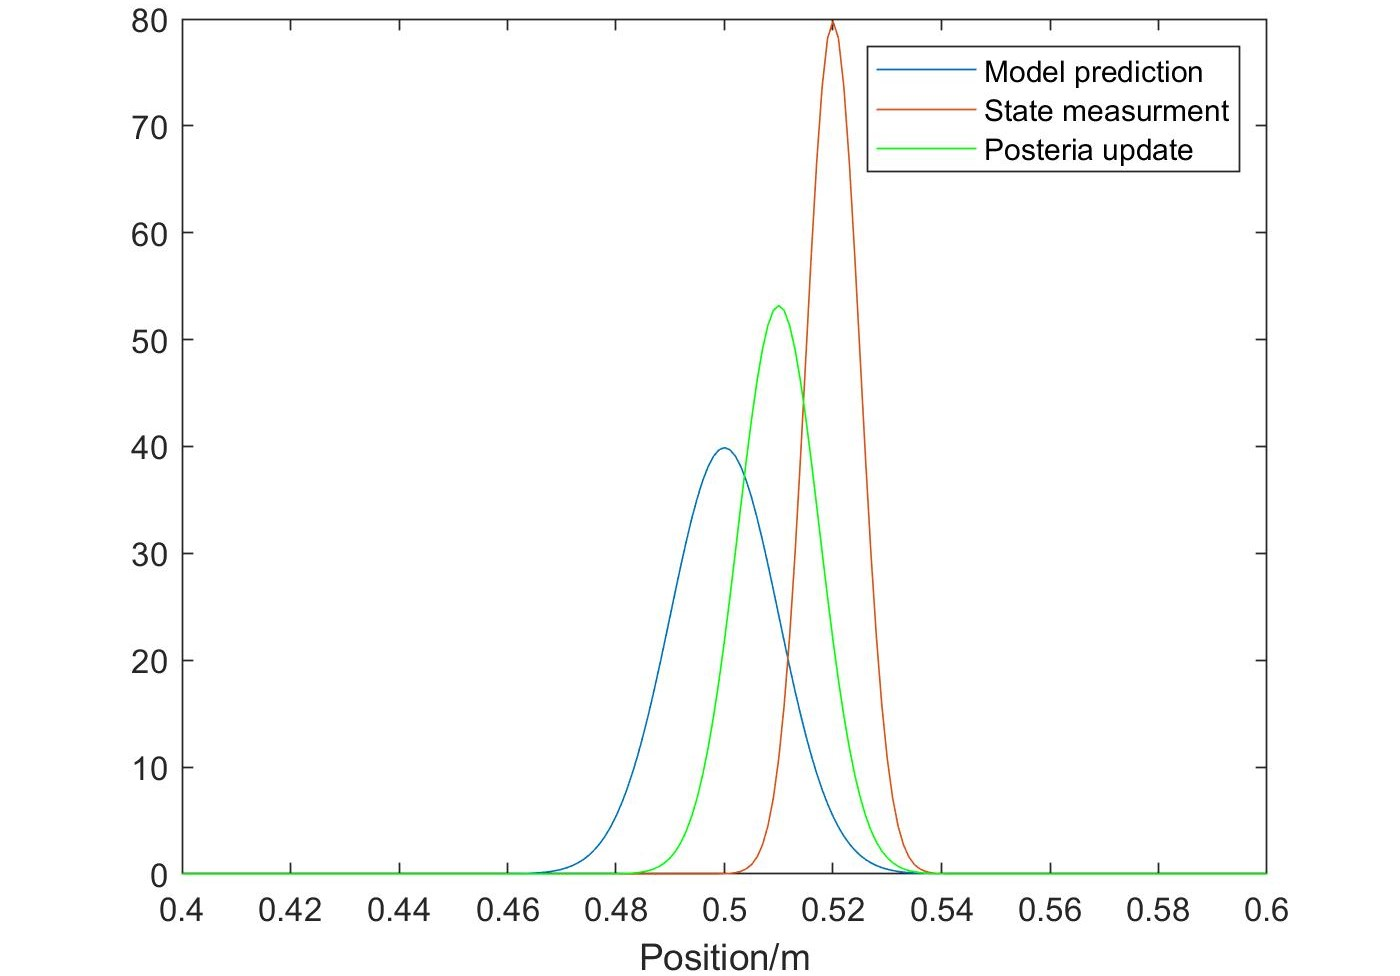
\includegraphics[width=\linewidth]{kalman}
  \caption{Kalman update step after a single step}
  \label{fig:kal}
\end{figure}
The updated estimate of position takes into account any dynamic drift present, as well as process and measurement noise and provides a better estimate of position then either method individually. This position can then be used to re-plan the trajectory of the next step in order to correct for any errors with the initial dynamics model. This means that the robot position can be accurately controlled, ensuring the real trajectories will match the desired one, and therefore allow successful completion of the task.


%------------------------------------------------------
\section{Question 4}
\subsection{Changes required}
As well as the changes listed above additional modifications were necessary for stairs.
\begin{itemize}
\item Change link lengths to be $[L_0, L_1, L_2, L_3, L_4, L_5]$ = [0.155, 0.118, 0.153, 0.153, 0.118, 0.125]m.
\item A mass was added to the leading foot. This was to allow the robot to shift the COM from the lower foot to the upper foot when taking a step.
\end{itemize}
One of the most interesting changes made was to the link lengths. The top sections were extended to allow for enough range to climb the tallest steps. However, it wasn't so simple when shortening the feet as a trade-off between balance maximum stride length and ability to overcome obstacles had to be made.  During a string the CoM moves, it's at the furthest away point from the stationary foot when the top links, and leading foot are straight and parallel to the ground. This also corresponds to a longer stride. If we assume the leading foot is maintained in an upright position and mass is symmetric across the robot, you can work out that the foot length must be at least half the total stride and stance length. In the  real robot this is a length of 15.3cm. If strides were reduced in length you could have smaller feet and increased stability. Adding a mass onto the leading foot shifted the CoM to be more forward, this means the two feet can be different lengths. Reducing the foot length has the downside of smaller strides but proved essential for tackling the stairs. Shorter feet were less likely to crash into the steps, therefore making route planning easier. The smaller foot print also allowed better balance on top of a stair, and repositioning for climbing the next step.  

\subsection{Planning Algorithm}
The same planning technique using inverse kinematics was implemented for the stairs. Variations were required as climbing involved both vertical motion dependant on step height, and small horizontal steps upon each step. The speed of some movements was varied to reduce the effect of toppling. Figure \ref{fig:stair} shows the stages for a 5 and 9cm stair. As can be seen in the images the initial three stages are identical for all step heights. Its only when the leading foot comes down that the trajectories differ. 

\begin{figure}[h]
  \centering
  \begin{subfigure}[t]{0.5\textwidth}
    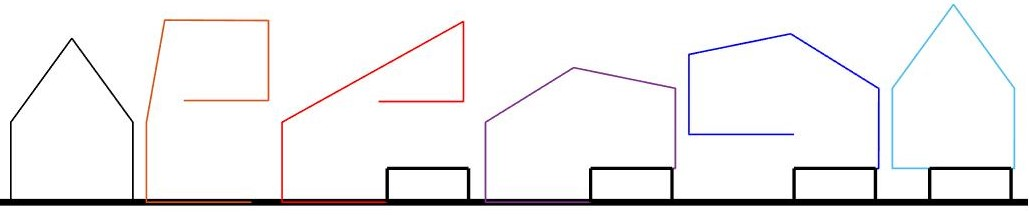
\includegraphics[width=\linewidth]{stepstages}
  \caption{5cm}
  \label{fig:stair5}
  \end{subfigure}
  \begin{subfigure}[t]{0.5\textwidth}
    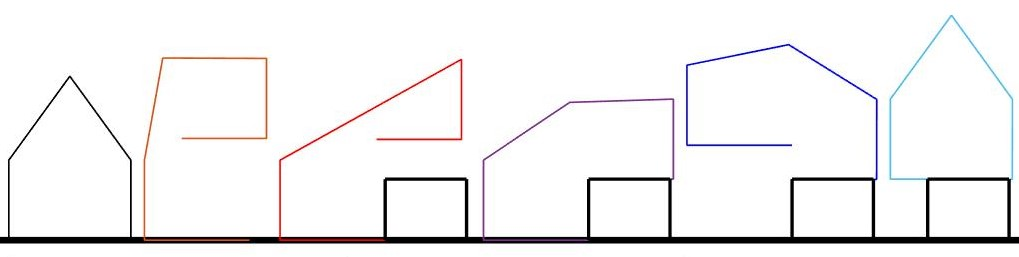
\includegraphics[width=\linewidth]{stepstages9}
  \caption{9cm}
  \label{fig:stair9}
  \end{subfigure}
  \caption{Intermediate stages for a given step height}
  \label{fig:stair}
\end{figure}
\begin{figure*}[h]
  \centering
    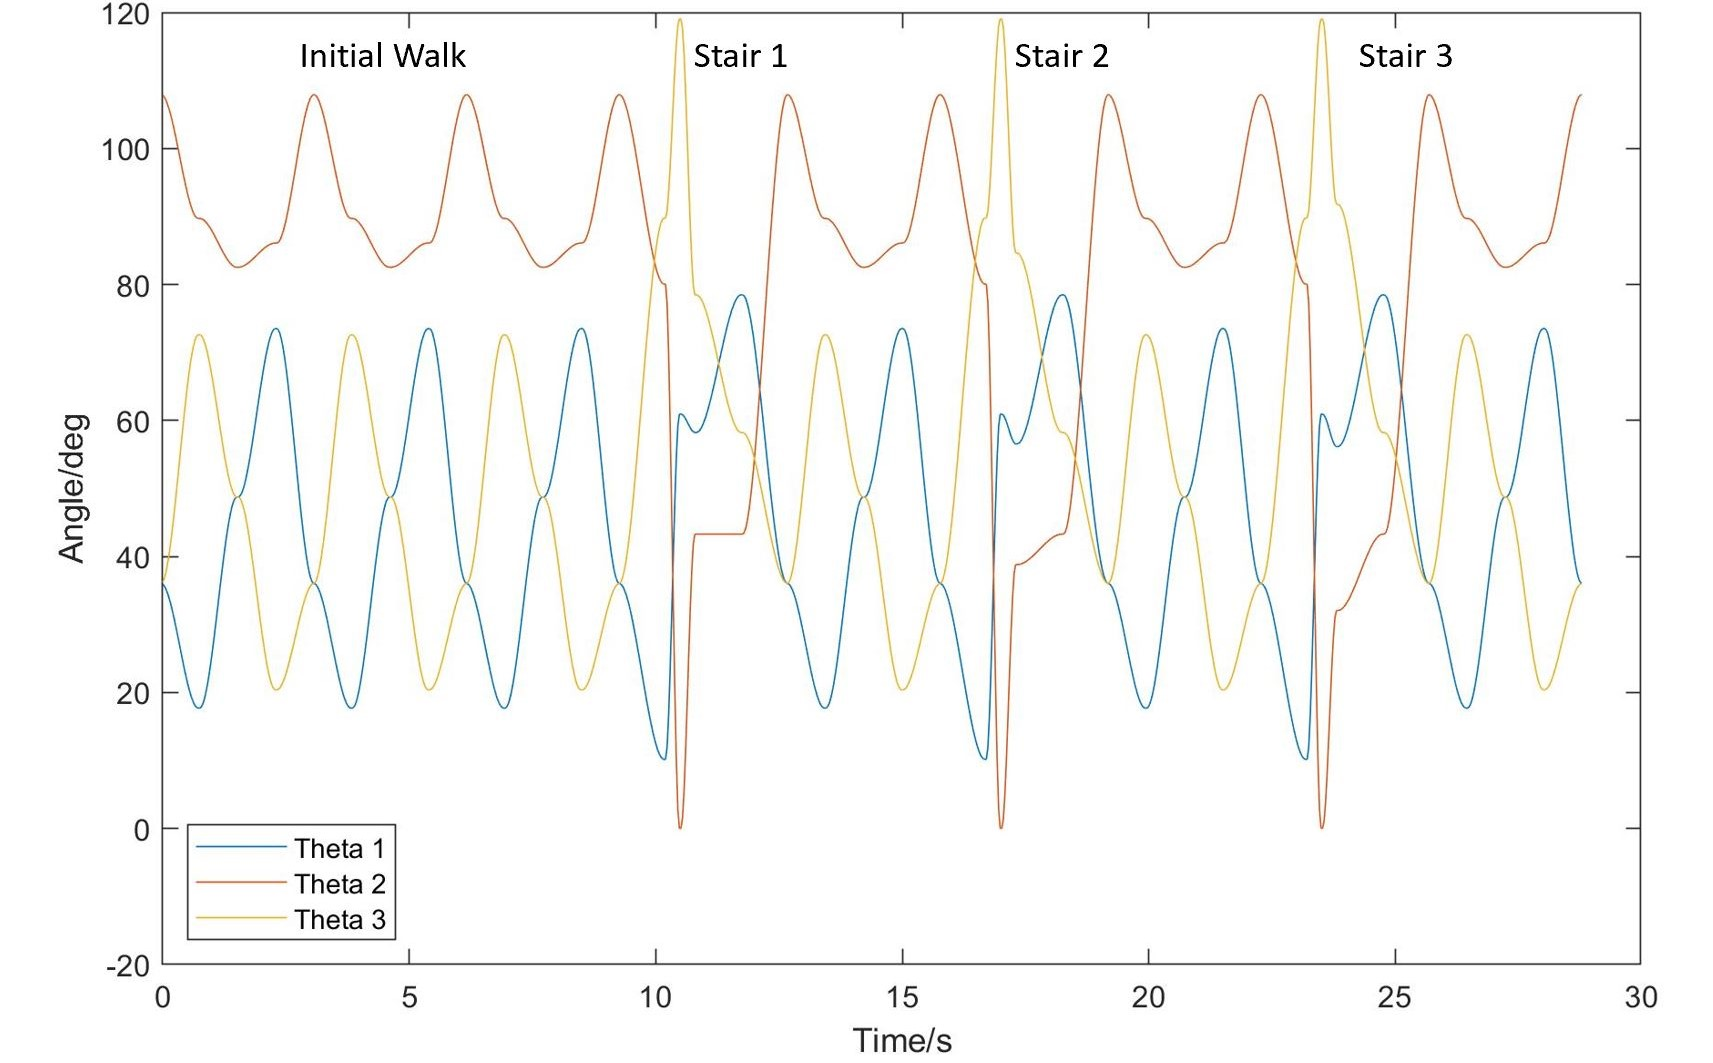
\includegraphics[width=0.96\linewidth]{steptraj}
  \caption{Joint angle trajectories for a the set of stairs}
  \label{fig:stj}
\end{figure*}
Third order polynomial fitting was once again used to interpolate smoothly between the stages. However, an additional check was required this time to ensure the robot didn't collide with the step as it moved.
\newline
When moving the leading foot forward the CoM must first reside above the foot not on the step. This means that at some point when moving the leading foot forward the CoM will shift to be above the stair and therefore not above the support polygon. This causes the robot to begin to tilt forward. To reduce the uncertainty stages 2-4 from figure \ref{fig:stair} were performed quickly to limit the motion caused by toppling. 
\newline
Once the robot had mounted a step it was required to take a small step forward to become level with the next step. Being level with the next step helps to reduce the accumulation of error as the robot moves. This step used the same process as question 2, with a step size of 5cm. Feedback could be introduced at this stage to measure the actual position on the step in order to calculate accurately the step size required. This would eliminate the uncertainty that is caused by unexpected slipping of feet during motion.
\newline
Figure \ref{fig:stj} shows the joint trajectories of the whole task. The fast stages can clearly be seen as well as the difference in movement between each step height.

Some additional factors were considered when planning the joint trajectories. These were motor torques and energy usage. The torque exerted on each motor can be treated as primarily static torque, dynamic torque can be ignored as angular accelerations are small throughout most of the motion. Static torque is the weight x moment arm. This is maximised in motors 1 when the top two links and the leading foot are parallel to the ground. Using a mass of 0.15kg per link and 0.25kg for the front mass an estimate of this maximum can be calculated as 2.03Nm (1.65Nm with link 4 vertical). This is relatively high meaning extending the arms this far should be reduced in order to conserve energy and stay within motor limits. This means that the shorter steps being implemented are useful for energy efficiently as well as balance.
\newline
Another factor to minimise is total energy usage. This is calculated by integrating the product of motor toques and angular accelerations. To minimise this these two factors were to be reduced where possible. This resulted in smaller steps and slower movements being desirable. The one exception to this was a fast move required to minimise the effect of toppling.
\subsection{Real world differences}
A lot of the differences in the real model compared to simulations were to do with assumptions taken when simulating. The following differences were observed and their effect was minimised by the changes mentioned earlier.
\begin{itemize}
\item Feet bent when taking a step, causing the front foot to land earlier then predicted.
\item The motors had a few degrees of wobble which caused the same problem as bending feet.
\item Non slip condition of feet was not true in practice.
\end{itemize}
These problems were possible to correct for or reduce in either mechanical redesigns or adjusting the calculated trajectories. The main problem was that the system dynamics played a very large role on the robot, and overall determined whether the trajectories would be followed correctly. 
\newline
In simulations the CoM calculations weren't exact which proved vital when balancing the robot while climbing stairs. The kinematic approach didn't account for any of the problems encountered. Using a dynamic model throughout the planning process would have solved this issue. However, due to the extra complexity and need for this model to be accurate it wasn't implemented when the task was undertaken. Instead measures were made to reduce the effects of the dynamics.
%----------------------------------------------
\subsection{Performance}
At the project competition our robot was unable to climb all the stairs. It was able to climbing 1-2 steps on occasion. With a few small tweaks to the planning algorithm and increasing the accuracy of our modelling the robot showed signs of being able to climb successfully. The major problem to overcome was accurately and reliably positioning the front foot upon each stair in a position it could balance. This proved unreliable due to slip varying between trials and therefore causing different positions of varying success to happen.
%------------------------------------------
\section{Future additions}
If more time were available before the competition there are various changes we'd have implemented after implementing the small tweaks necessary to get the current model working.
\subsection{Dynamic model}
The first change would would be to design the trajectories using a dynamic model. This would increase the task complexity greatly, but has the advantage of faster and more efficient movement possible compared to a purely kinematic approach. This is because the problem is inherently dynamic and the dynamics plays a vital role in predicting robot movement reliably. Being able to accurately predict robot behaviour means that a joint planning algorithm can correctly determine how the robot will balance at each point in the motion, and therefore successfully optimise the joint trajectory.
The additional requirements for a dynamics model are the following:
\begin{itemize}
\item Accurate mass distribution of the robot, including the moment of inertia of the robot for given joint angles.
\item Forces and accelerations of and within each robot section.
\item The stiffness of components in order to model bending accurately.
\item Uncertainty in angular position of motors under load.
\item Motor torques, friction and damping
\item Coefficient of friction between surfaces.
\end{itemize}

\subsection{Trajectory optimisation}
Trajectory optimisation is important as it can ensure that energy is minimised throughout the motion while still maintaining a stable and repeatable path. The method currently implemented used polynomial fitting between stages in order to reduce factors such as angular acceleration. With the choice of these intermediate points minimising joint torques throughout motion. Both these factors help to optimise trajectory. By further discretizing the space between start and end points of each step the trajectory could be better optimised. Additional discretization would increase computational time but allow efficent travel. This method would follow the steps below.
\begin{itemize}
\item Discretize the configuration space, with smaller units located around places of interest such as the stairs.
\item Define a start and end position for a step.
\item Define objectives to minimise such as motor torque.
\item Define constraints, such as balance and obstacle interference.
\item Perform a search algorithm through the defined space in order to minimise your objective and find an optimum trajectory
\end{itemize}

%------------------------------------------------------------
\onecolumn
\section{Appendix}
\begin{equation}
\begin{bmatrix}
x_5 \\
y_5
\end{bmatrix}
=
\begin{bmatrix}
x_1 \\
y_1
\end{bmatrix}
+
\begin{bmatrix}
L_2Sin(\theta_1)+L_3Sin(\theta_1+\theta_2)+L_4Sin(\theta_1+\theta_2+\theta_3) \\
L_1 + L_2Cos(\theta_1)+L_3Cos(\theta_1+\theta_2)+L_4Cos(\theta_1+\theta_2+\theta_3)
\end{bmatrix}
\label{eq:fk}
\end{equation}  

\begin{equation}
\begin{bmatrix}
x_1 \\
y_1
\end{bmatrix}
=
\begin{bmatrix}
x_5 \\
y_5
\end{bmatrix}
+
\begin{bmatrix}
-L_3Sin(\theta_3)-L_2Sin(\theta_2+\theta_3)-L_1Sin(\theta_1+\theta_2+\theta_3) \\
L_4 + L_3Cos(\theta_3)+L_2Cos(\theta_2+\theta_3)+L_1Cos(\theta_1+\theta_2+\theta_3)
\end{bmatrix}
\label{eq:fk2}
\end{equation} 

\begingroup
\let\clearpage\relax 
\twocolumn 
\endgroup
\subsection{Code}

\begin{lstlisting}[language=matlab]
function robot_walk(walker)
s=arduino()
% 
sv1 = servo(s, 'D9', 'MinPulseDuration', 700*10^-6, 'MaxPulseDuration', 2300*10^-6);
...

traj = walker.th;

convert to be lines up with the robot
traj = (traj + [7;7;20])/160;
traj(3,:)=1-traj(3,:);


T= (walker.t(2)-walker.t(1));
m=20;
to_start = zeros(3,m);
for i = 1:3
    to_start(i,:) = linspace(currentpos(i),traj(i,1),m);
end    
traj = cat(2,to_start,traj);

for i = 1:size(traj,2)
    writePosition(sv1, traj(1,i));
    writePosition(sv2, traj(2,i));
    writePosition(sv3, traj(3,i));

    
    %fprintf('Current motor position is %d degrees\n', angle);
    pause(T);
end
end
\end{lstlisting}
\newpage
\vphantom{500mm}
\vspace{25mm}

\begin{lstlisting}[language=matlab]
function walker = cw2_main()

global L0 L1 L2 L3 L4 L5 thub thlb

%% Initialisation and Limits
%sim_type = 'real'
sim_type = 'real';

switch sim_type
    case 'real'
        ....
    case 'CW'
    	....
end

% joint actuation limits
thub = [151 157 145]';
thlb = [-29 -23  -35]';
th0 = [60; 60; 60];

%% start position
xy1start = [0; 0];
xy5start = [0.18; 0];
groundpoint = 1;
thstart = walker_inv_kin(th0, xy1start, xy5start, 1);
xyrobotstart  = walker_fw_kin(thstart, xy1start, 1);

tstart = 0;
tstep = 3;
tend = tstart + tstep;

%% Step Length
% max step length
maxstep_th = walker_inv_kin(th0, xy1start, (xy1start + [1;0]), 1);
maxstep_xyrobot  = walker_fw_kin(maxstep_th, xy1start, 1);
max_steplength = maxstep_xyrobot(1,5) - xy5start(1);

% specified step length
steplength =0.05; %0.105;

if steplength > max_steplength
    disp('step size too large! Using max step size instead')
    steplength = max_steplength;
end

%% Initialisation
....

%% approach first step
first_steps = 3;

for i = 1:first_steps
   ......
end

%% horizontal and vertical steps
steplengths = [0.10, 0.10, 0.10];
stepheights = [0.05, 0.07, 0.09];

no_steps = 3;
%while tend < 10
for i = 1:no_steps
    %% generate vertical step
    [xy1end, xy5end, stages]...
        = vstep_stages(thstart, xy1start, xy5start, steplengths(i), stepheights(i));
    
    % joint trajectories
    [th, gnd, xy1, xy5, t] = joint_trajectories(stages, tstart, tend);
    
    % save data
    ......
    
    % iterate
    tend = tstart + tstep;
    xy1start = xy1end;
    xy5start = xy5end;
    thstart = th(:,end);
    
    %% generate horizontal step
    .......
end

end


function xyrobot = walker_fw_kin(th, xyground, groundpoint)
%% Forward kinematics of walker
global L1 L2 L3 L4

th1 = th(1);
th2 = th(2);
th3 = th(3);

%% which leg is on the ground?
if groundpoint == 1
    % xy1 on ground
    xy1 = xyground;
    xy2 = xy1 + [0; L1];
    xy3 = xy2 + L2*[sind(th1); cosd(th1)];
    xy4 = xy3 + L3*[sind(th1 + th2); cosd(th1 + th2)];
    xy5 = xy4 + L4*[sind(th1 + th2 + th3); cosd(th1 + th2 + th3)];
else
    % xy5 on ground
    xy5 = xyground;
    xy4 = xy5 + [0; L4];
    xy3 = xy4 + L3*[-sind(th3); cosd(th3)];
    xy2 = xy3 + L2*[-sind(th2 + th3); cosd(th2 + th3)];
    xy1 = xy2 + L1*[-sind(th3 + th2 + th1); cosd(th3 + th2 + th1)];
    xyrobot = [xy1, xy2, xy3, xy4, xy5];
    xy1;
end
xyrobot = [xy1, xy2, xy3, xy4, xy5];

end

function th = walker_inv_kin(thstart, xy1, xy5, groundpoint)
%% find inverse kinematics, usindg an fsolve non-linear solving algorithm
global thlb thub

fun = @(th_try)err_walker_inv_kin(xy1,xy5,th_try, groundpoint);

options = optimset('Display','off', 'TolFun', 1e-7);
th = lsqnonlin(fun, thstart, thlb, thub, options);

end

function err = err_walker_inv_kin(xy1, xy5, th, groundpoint)
%% solver function for inverse kinematics

% error between desired xy and current tried xy
if groundpoint == 1
    % find xy5
    xyfor = walker_fw_kin(th, xy1, groundpoint);
    err = xy5 - xyfor(:,5);
else
    % find xy1
    xyfor = walker_fw_kin(th, xy5, groundpoint);
    err = xy1 - xyfor(:,1);
end
err2 = 180 - (th(1) + th(2) + th(3));
err = [err; err2];
end

function [th_t,gnd_t, xy1_t, xy5_t, t] = joint_trajectories(stages, tstart, tend)
%% fit polynomial trajectory to points specified by stages struc
%% initialise
....

% number of points
total_npoints = 100;

%% fit sequential third-order polynomials
for i = 1:length(x)-1
    thA = stages.th(:,i);
    thB = stages.th(:,i+1);
    xA = x(i);
    xB = x(i+1);
    gndB = stages.gnd(i+1);
    npoints = round(total_npoints*stages.timefraction(i));
    
    % define polynomial coeffs
    a0 = thA;
    a1 = [0;0;0];
    a2 = 3*(thB - thA)/((xB-xA)^2);
    a3 = -2*(thB - thA)/((xB-xA)^3);
    
    % define ground point leg and position
    xAB = linspace(xA, xB, npoints) - xA;
    % remove first point to avoid duplicate timesteps
    if i == 1
        xAB(1) = [];
    end
    gndAB = gndB*ones(1, size(xAB, 2));
    if gndAB(1) == 1
        xygndAB = stages.xy1(:,i+1).*ones(2, size(xAB,2));
    else
        xygndAB = stages.xy5(:,i+1).*ones(2, size(xAB,2));
    end
    
    % calculate polynomial values
    th_t = [th_t, (a3*(xAB.^3) + a2*(xAB.^2) + a1*(xAB) + a0)];
    gnd_t = [gnd_t, gndAB];
    xygnd_t = [xygnd_t, xygndAB];
    t = [t, (xAB + xA)];
end
% calculate fw kinematics
....
end

\end{lstlisting}

%------------------------------------------------
\end{document}
